% !TEX root = 99_main.tex

% \begin{figure}
% \begin{center}
% 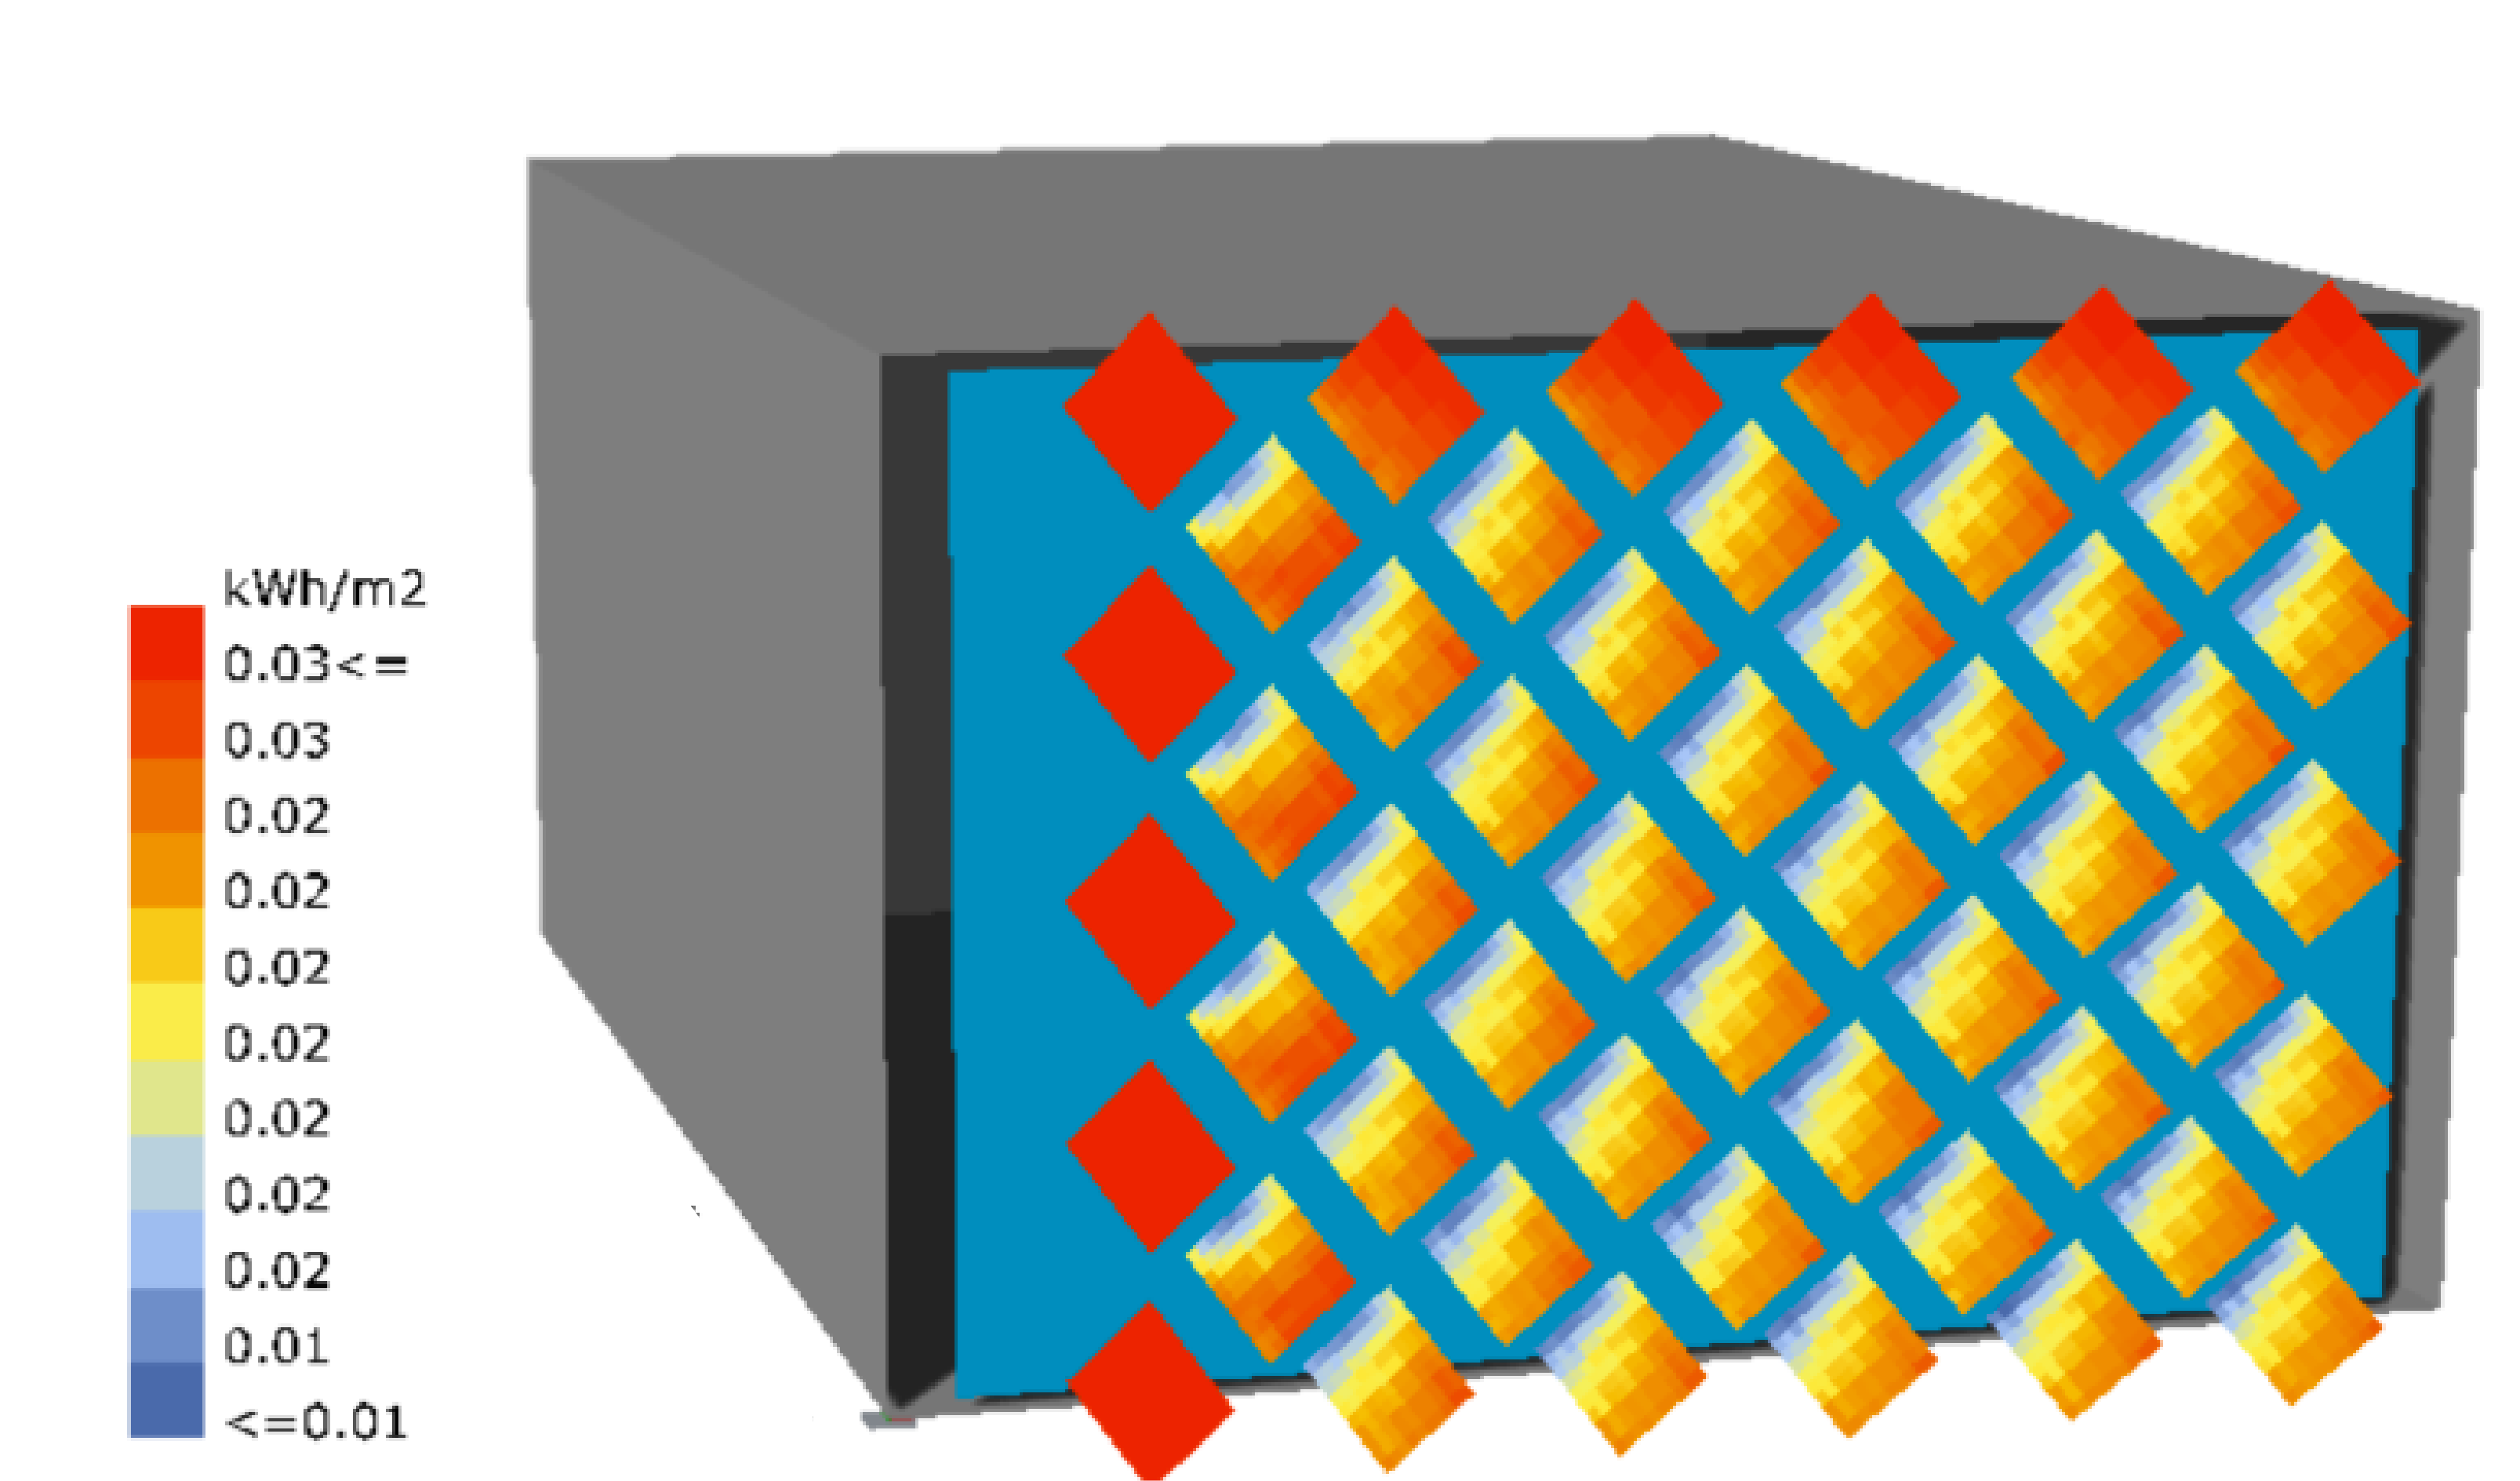
\includegraphics[width=8cm, trim= 0cm 0cm 0cm 0cm,clip]{radiationanalysis.png}
% \caption{Incident radiation on the PV panels. Light blue spots indicate areas of self shading}
% \label{fig:radiationanalysis}
% \end{center}
% \end{figure}


The optimal configurations of the ASF can be visualised using carpet-plots. Figure \ref{fig:carpetplot} details carpet-plots of the facade optimised to maximise PV generation\footnote{For this abstract, a constant efficiency of 0.072 was assumed for the PV electricity generation.}, and minimise heating, cooling and lighting demands independently. We can see how open configurations (light coloured) are chosen to minimise the building heating demands during the winter months and early mornings of spring and autumn. Likewise closed configurations (dark colours) are the preferred solutions to minimise the cooling demand during the summer months. Lighting control is only apparent during the twilight hours where the facade prefers an open position to avoid the use of artificial lighting. The PV optimisation follows a solar tracking model for most hours and as far as the limited range of angles allows. This causes some issues during twilight summer hours as the actuator cannot physically align itself normal to the sunlight. 




\begin{figure*}
\begin{center}
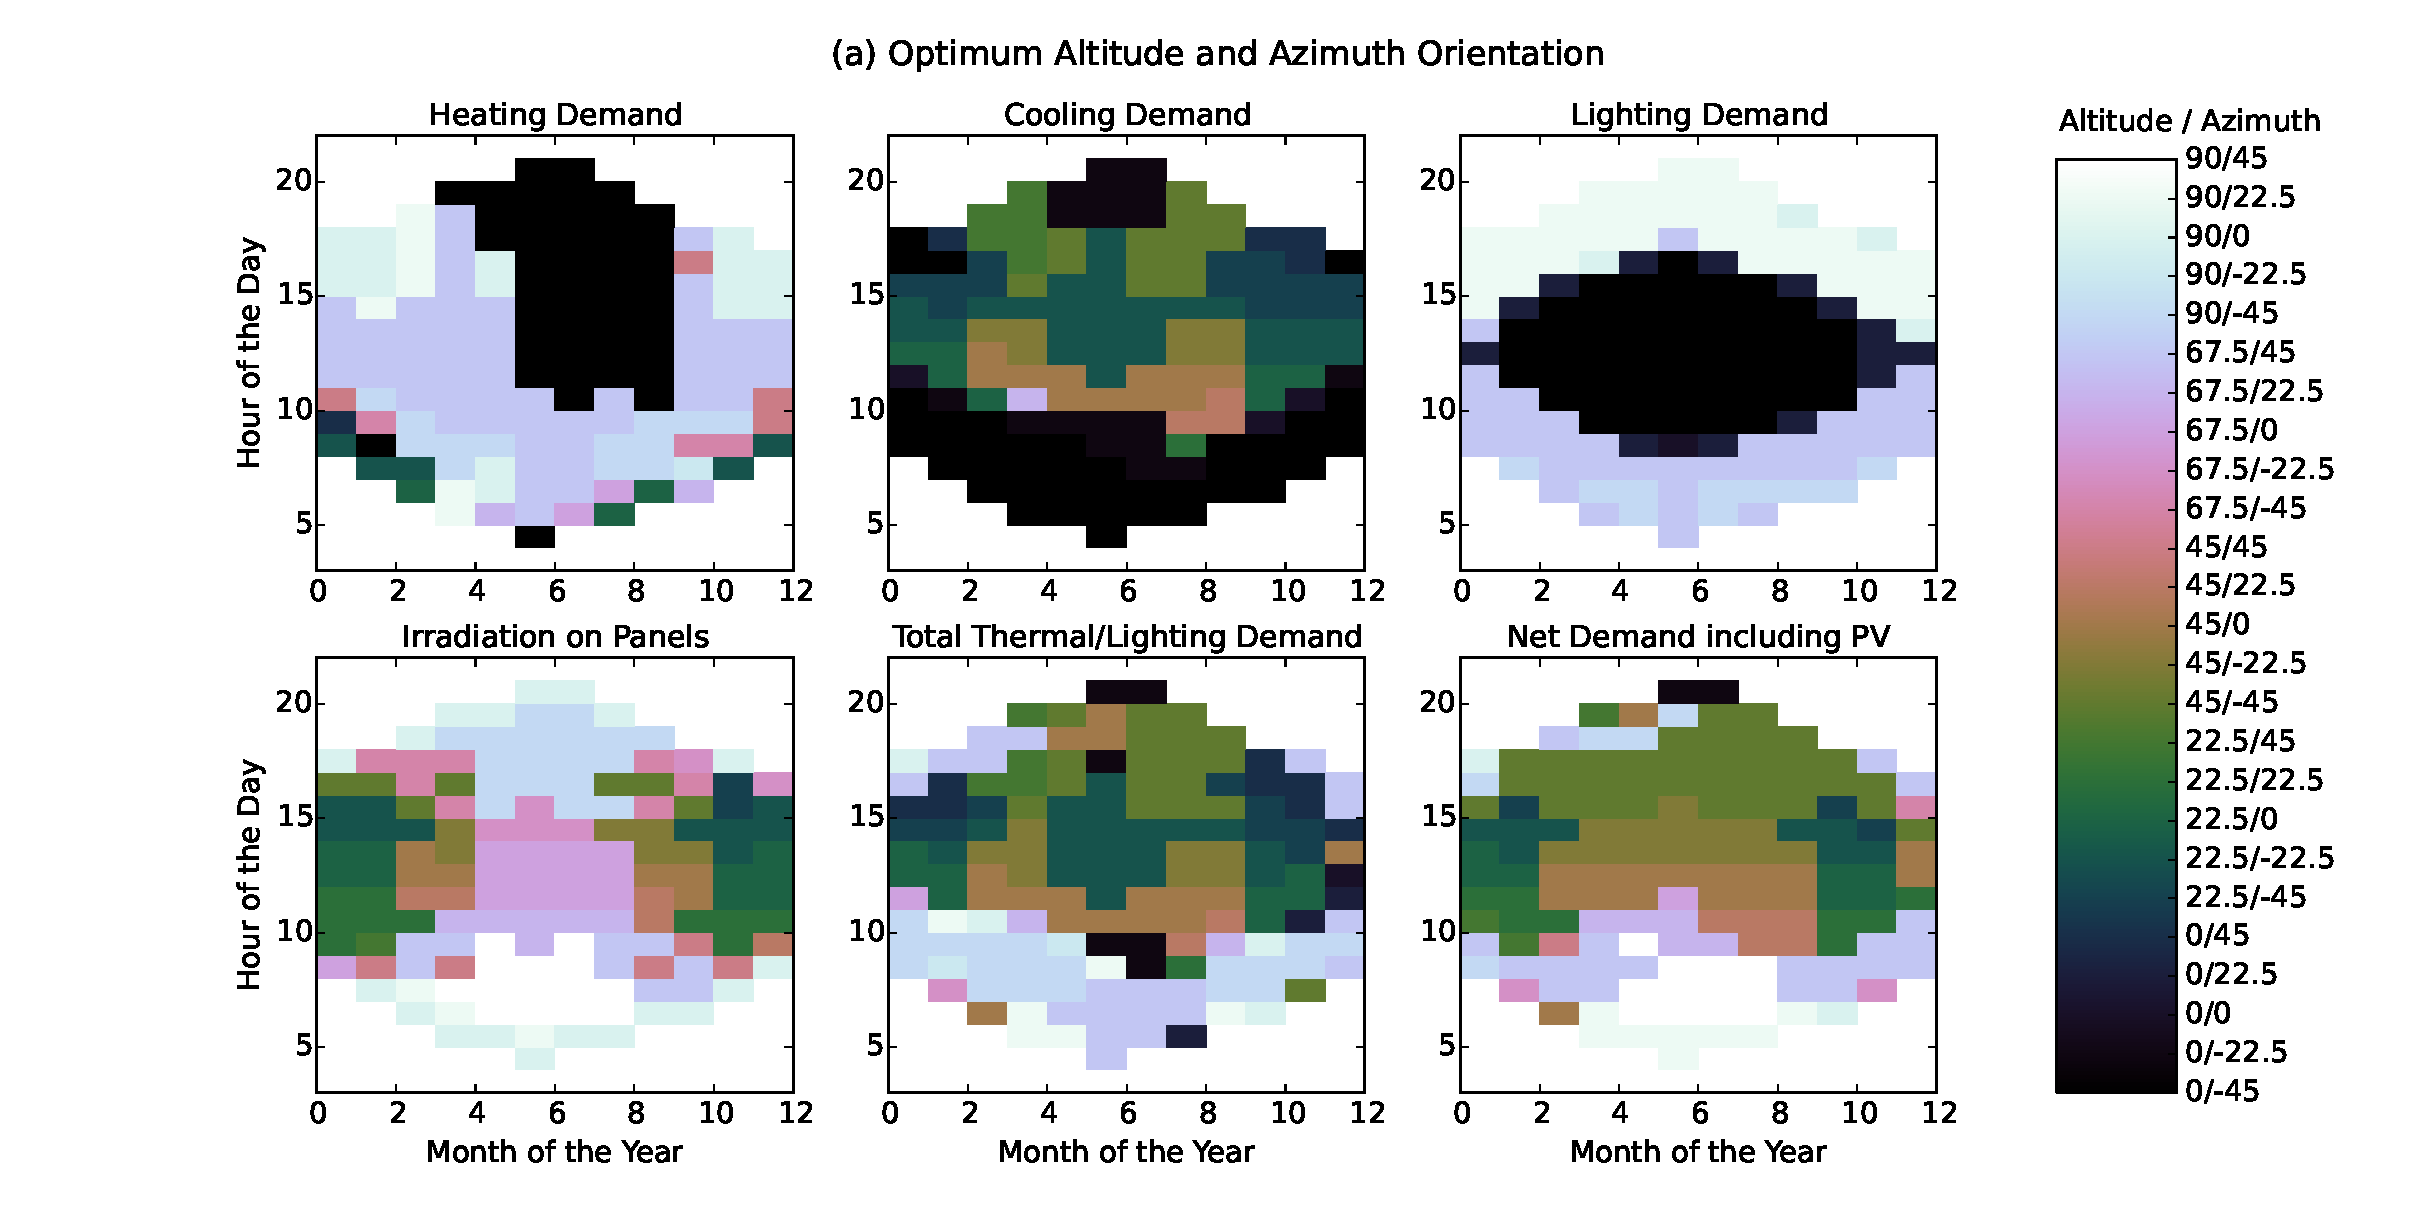
\includegraphics[width=17cm, trim= 0cm 0cm 0cm 0cm,clip]{carpetplot_angles.eps}
\caption{A carpet plot detailing the optimal configuration to minimise the (a) heating demand, (b) cooling demand, (c) lighting demand, and (d) maximise PV generation. Each configuration is represented by an angle of orientation around the x-axis (Altitude) and y-axis (Azimuth) as seen in the legend. Figure (e) details the combinations for optimum building thermal management without PV production. (f) also includes the PV production}
\label{fig:carpetplot}
\end{center}
\end{figure*}

\begin{figure*}
\begin{center}
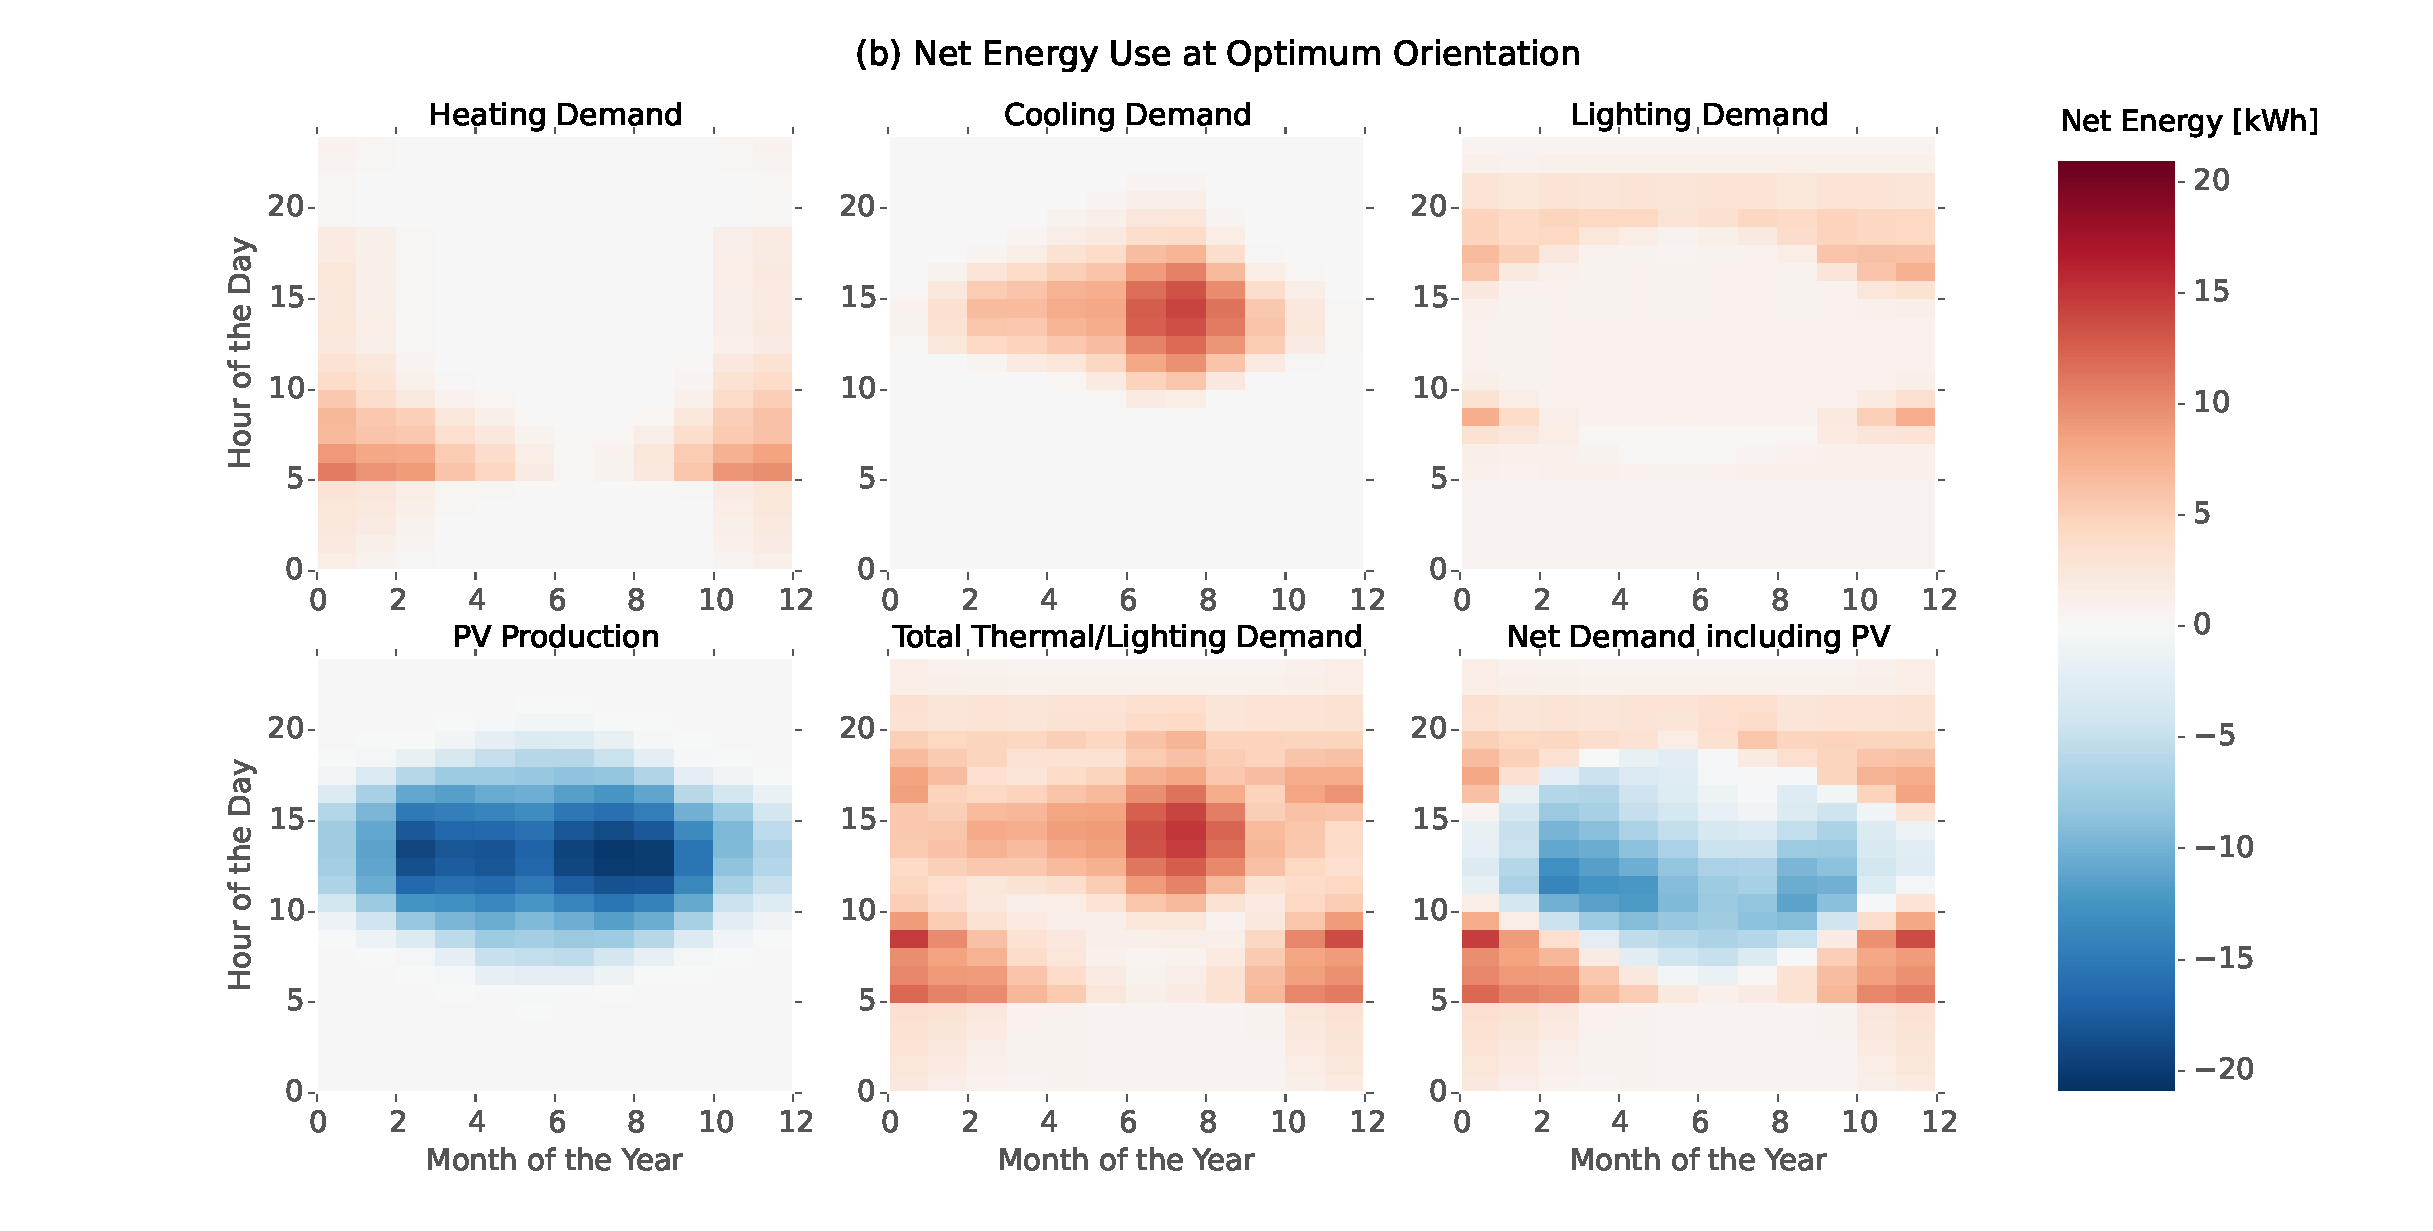
\includegraphics[width=17cm, trim= 0cm 0cm 0cm 0cm,clip]{carpetplot_energy.eps}
\caption{A carpet plot detailing the net energy consumption. Each square represents the total energy consumption for that specific hour of the entire month. Red colours detail the energy demand, while blue colours detail the energy supply.}
\label{fig:carpetplot_energy}
\end{center}
\end{figure*}



When the four optimisation cases are combined to achieve the configurations for total energy minimisation we get some interesting results. There is a conflict in the summer evenings between minimising lighting and cooling demands. Likewise, we also see a conflict between heating and PV production during the winter months. The overall energy optimization including PV electricity production shows a strong tendency to follow the optimal PV production pattern. This however changes if the building system becomes more inefficient. Less efficient heating for example would result in configurations optimised for heating overpowering those of PV electricity generation.


Figure \ref{fig:carpetplot_energy} shows the net energy use at these optimum angles. It is interesting to see how the combination of electricity generation and adaptive shading can compensate for the entire energy use during sunlit hours.

